\documentclass[11pt]{article}
\usepackage{enumerate}
\usepackage{fullpage}
\usepackage{fancyhdr}
\usepackage{amsmath, amsfonts, amsthm, amssymb}
\usepackage{color}
\usepackage[]{graphicx}

\setlength{\parindent}{0pt}
\setlength{\parskip}{5pt plus 1pt}
\pagestyle{empty}

\def\indented#1{\list{}{}\item[]}
\let\indented=\endlist

\newcounter{questionCounter}
\newcounter{partCounter}[questionCounter]
\newenvironment{question}[2][\arabic{questionCounter}]{%
    \setcounter{partCounter}{0}%
    \vspace{.25in} \hrule \vspace{0.5em}%
        \noindent{\bf #2}%
    \vspace{0.8em} \hrule \vspace{.10in}%
    \addtocounter{questionCounter}{1}%
}{}
\renewenvironment{part}[1][\alph{partCounter}]{%
    \addtocounter{partCounter}{1}%
    \vspace{.10in}%
    \begin{indented}%
       {\bf (#1)} %
}{\end{indented}}

%%%%%%%%%%%%%%%%%%%%%%%HEADER%%%%%%%%%%%%%%%%%%%%%%%%%%%%%%
\newcommand{\myname}{Shashank Singh}
\newcommand{\myandrew}{sss1@andrew.cmu.edu}
\newcommand{\myclass}{86-595 Neural Data Analysis}
\newcommand{\myhwnum}{1}
\newcommand{\duedate}{Tuesday, September 18, 2012}
%%%%%%%%%%%%%%%%%%%%%%%%%%%%%%%%%%%%%%%%%%%%%%%%%%%%%%%%%%%

%%%%%%%%%%%%%%%%%%%%CONTENT MACROS%%%%%%%%%%%%%%%%%%%%%%%%%
\newcommand{\be}{\begin{enumerate}}
\newcommand{\ee}{\end{enumerate}}
\renewcommand{\qed}{\quad $\blacksquare$}
\newcommand{\mqed}{\quad \blacksquare}
\newcommand{\inv}{^{-1}}
\newcommand{\bx}{\mathbf{x}}
\newcommand{\by}{\mathbf{y}}
\newcommand{\bff}{\mathbf{f}}
\newcommand{\bzero}{\mathbf{0}}
\newcommand{\N}{\mathbb{N}} % natural numbers
\newcommand{\Q}{\mathbb{Q}} % rational numbers
\newcommand{\R}{\mathbb{R}} % real numbers
\newcommand{\E}[1]{\mathsf{E}\left[#1\right]} % expected value
\newcommand{\Var}[1]{\mathsf{Var}\left[#1\right]} % variance
\newcommand{\Poisson}[1]{\operatorname{Poisson}\left(#1\right)} % Poisson distribution
\newcommand{\Exp}[1]{\operatorname{Exp}\left(#1\right)} % Exponential distribution
\newcommand{\U}[2]{\operatorname{U}\left(#1,#2\right)} % Uniform distribution
%%%%%%%%%%%%%%%%%%%%%%%%%%%%%%%%%%%%%%%%%%%%%%%%%%%%%%%%%%%

\begin{document}
\thispagestyle{plain}

{\Large Homework \myhwnum} \\
\myclass \\
Name: \myname \\
Email: \myandrew \\
Due: \duedate \\
\begin{question}{Problem 1}
Suppose that $X \sim \Poisson{\lambda}$, and recall that $\E{X} = \lambda$.
\begin{align*}
\E{X^2}
 & = \sum_{i = 1}^{\infty} i^2\cdot P(X = i)
   = \sum_{i = 1}^{\infty} i\cdot \frac{\lambda^i}{(i - 1)!}e^{-\lambda} \\
 & = \sum_{i = 0}^{\infty} (i + 1)\cdot \frac{\lambda^{i + 1}}{i!}e^{-\lambda} & \mbox{(re-index the summation)}\\
 & = \lambda\left(\sum_{i = 0}^{\infty} i \cdot \frac{\lambda^i}{i!}e^{-\lambda}
   + \sum_{i = 0}^{\infty} \frac{\lambda^i}{i!}e^{-\lambda}\right) \\
 & = \lambda\left(\E{X} + e^{\lambda}e^{-\lambda}\right) & \mbox{(def. of $\E{X}$, Taylor series for $e^{\lambda}$)}\\
 & = \lambda\left(\lambda + 1\right) = \lambda^2 + \lambda.
\end{align*}
Therefore,
\[\Var{X} = \E{X^2} - \E{X}^2 = \lambda^2 + \lambda - \lambda^2 = \lambda = \E{X}. \mqed\]
\end{question}

\begin{question}{Problem 2}
$\forall n \geq 0$, $P(Z = n)$ is the number of ways of satisfying
$X_1 + X_2 = n$, times the probability that $X_1$ and $X_2$ satisfy that
equation:
\[P(Z = n)
 = \sum_{i = 0}^n \binom{n}{i} P(X_1 = i \cap X_2 = n - i)
 = \sum_{i = 0}^n \binom{n}{i} P(X_1 = i)P(X_2 = n - i)
\]
(the binomial coefficient comes from the fact that, of the $n$ spikes, any $i$
may have come from the first neuron, and the second equality follows from the
independence of $X_1$ and $X_2$). Therefore,
\begin{align*}
P(Z = n)
 & = \sum_{i = 0}^n \binom{n}{i}
              \left(\frac{\lambda_1^i}      {i!}      e^{-\lambda_1}\right)
              \left(\frac{\lambda_1^{n - i}}{(n - i)!}e^{-\lambda_1}\right) \\
 & = \frac{e^{-(\lambda_1 + \lambda_2)}}{n!}
                        \sum_{i = 0}^n \binom{n}{i}
                                    \lambda_1^i\lambda_2^{n - i}
   = \frac{(\lambda_1 + \lambda_2)^n}{n!}e^{-(\lambda_1 + \lambda_2)}
                                            & \mbox{(by the Binomial Theorem)}
\end{align*}
Therefore, $Z \sim$ \fbox{$\Poisson{\lambda_1 + \lambda_2}$.}
\end{question}

\begin{question}{Problem 3}
Let $X \sim \Poisson{\lambda}$ be the number of spikes, and let $Z$ be the
number of spikes we detect. The value of $Z | X$ is distributed binomially
(for each spike, we flip a coin biased to be heads with probability $0.9$,
and count the number of heads). Thus, by the Law of Total Probability,
$\forall n \in \N$, if $p = 0.9$,
\begin{align*}
P(Z = n)
 & = \sum_{i = n}^{\infty} P(X = i) \cdot P(Z = n | X = i) & \mbox{(since $Z \leq X$)} \\
 & = \sum_{i = n}^{\infty} \frac{\lambda^i}{i!}e^{-\lambda} \binom{i}{n}p^n(1 - p)^{i - n} \\
 & = \sum_{i = n}^{\infty} \frac{\lambda^i}{i!}e^{-\lambda} \frac{i!}{n!(i - n)!}p^n(1 - p)^{i - n} \\
 & = \sum_{i = 0}^{\infty} \lambda^{i + n}e^{-\lambda} \frac{p^n(1 - p)^i}{n!i!} & \mbox{(re-index summation)}\\
 & = \frac{(p\lambda)^n}{n!}e^{-\lambda}\sum_{i = 0}^{\infty} \frac{((1 - p)\lambda)^i}{i!} & \mbox{(factor out constants)}\\
 & = \frac{(p\lambda)^n}{n!}e^{-\lambda}e^{(1 - p)\lambda}
   = \frac{(p\lambda)^n}{n!}e^{p\lambda}. & \mbox{(Taylor series for exponential)}
\end{align*}
Therefore, $Z \sim$ \fbox{$\Poisson{p\lambda}$.}
\end{question}

\begin{question}{Problem 4}
Since $V \sim \mathcal{N}(\upsilon + b,\sigma^2)$,
$X := (V - \upsilon) \sim \mathcal{N}(b,\sigma^2)$. Thus,
\[\E{X^2} = \Var{X} + \E{X}^2 = \mbox{\fbox{$\sigma^2 + b^2$.}}\]
(Isn't this true of any estimator?)
\end{question}

\begin{question}{Problem 5}
\begin{enumerate}[a.]
\item $\forall t \in \R$, $F(t)$ is the probability that the cue has occurs
before time $t$, so that $1 - F(t)$ is the probability that the cue occurs
after time $t$, and $f(t)$ is the probability that the cue occurs in the
infinitesimal increment of time after $t$. Thus, at any given moment in time
$t$, the probability of getting the cue given that it hasn't already occured
is
\[P(\mbox{cue now} | \mbox{no cue yet})
 = \frac{P(\mbox{cue now} \wedge \mbox{no cue yet)}}{P(\mbox{no cue yet})}
 = \frac{P(\mbox{cue now})}{P(\mbox{no cue yet})}
 = \frac{f(t)}{1 - F(t)}. \mqed
\]
\item The hazard function of the exponential distribution $\Exp{\mu}$ is
\[\lambda_e(t)
 = \frac{\mu e^{-\mu t}}{e^{-\mu t}}
 = \mu.
\]
For $t \in (a,b)$, the hazard function of the uniform distribution
distribution $\U{a}{b}$ is
\[\lambda_u(t)
 = \frac{\left( \frac{1}{b - a} \right)}{\left( \frac{t - a}{b - a} \right)}
 = \frac{1}{t - a}.
\]
Since $\lambda_{e}$ is constant whereas $\lambda_{u}$ is strictly increasing
(or constant $0$), the subject cannot prepare for an exponentially distributed
cue time, whereas, with a uniformly distributed cue time, the subject would
become increasing expectant of a cue over time (in fact, theres a $3$-line
proof that the exponential distribution is the \emph{only} nice distribution
with a constant hazard function). Thus, the exponential distribution is better.
\end{enumerate}
\end{question}

\begin{question}{Problem 6}
\begin{enumerate}[a.]
\item $\rho_f \approx 0.1728$. See Figure~\ref{fig:6a}.
\begin{figure}[h]
\begin{center}
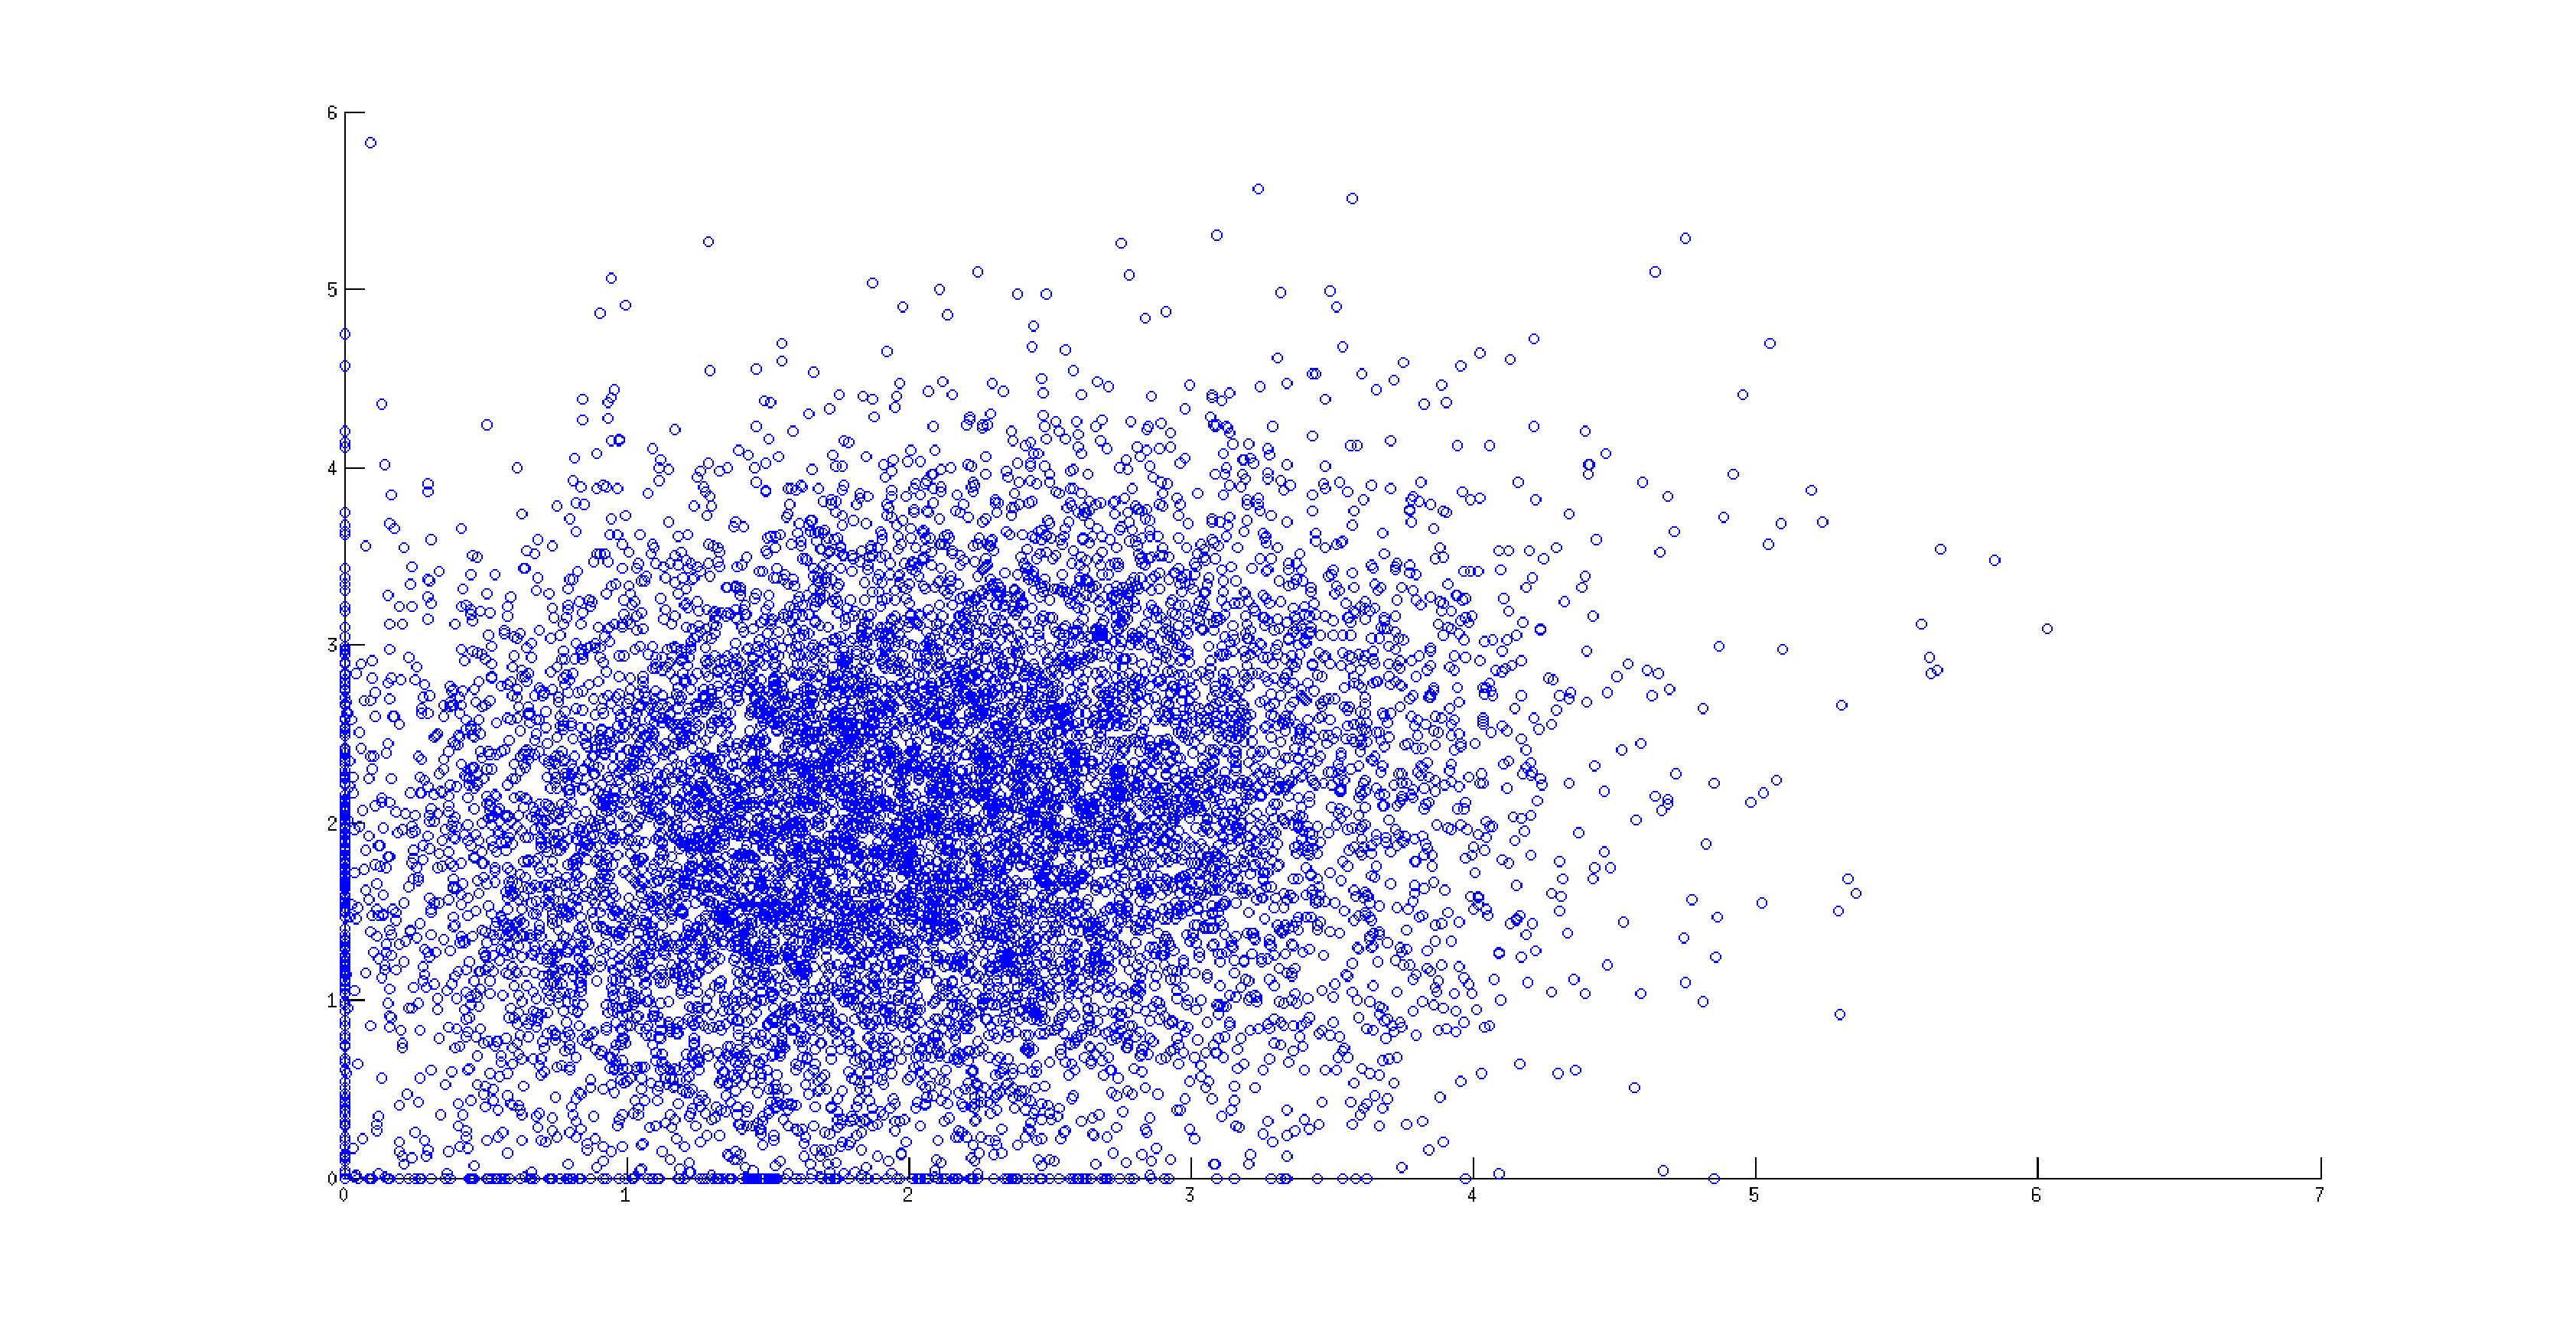
\includegraphics[width=0.9\textwidth]{6a}
\end{center}
\caption{Scatter plot of $f_2$ over $f_1$, for $\mu = 2,\rho_v = 0.2$.}
\label{fig:6a}
\end{figure}
\newpage

\item $\rho_f \approx 0.0203$. See Figure~\ref{fig:6b}.
\begin{figure}[h]
\begin{center}
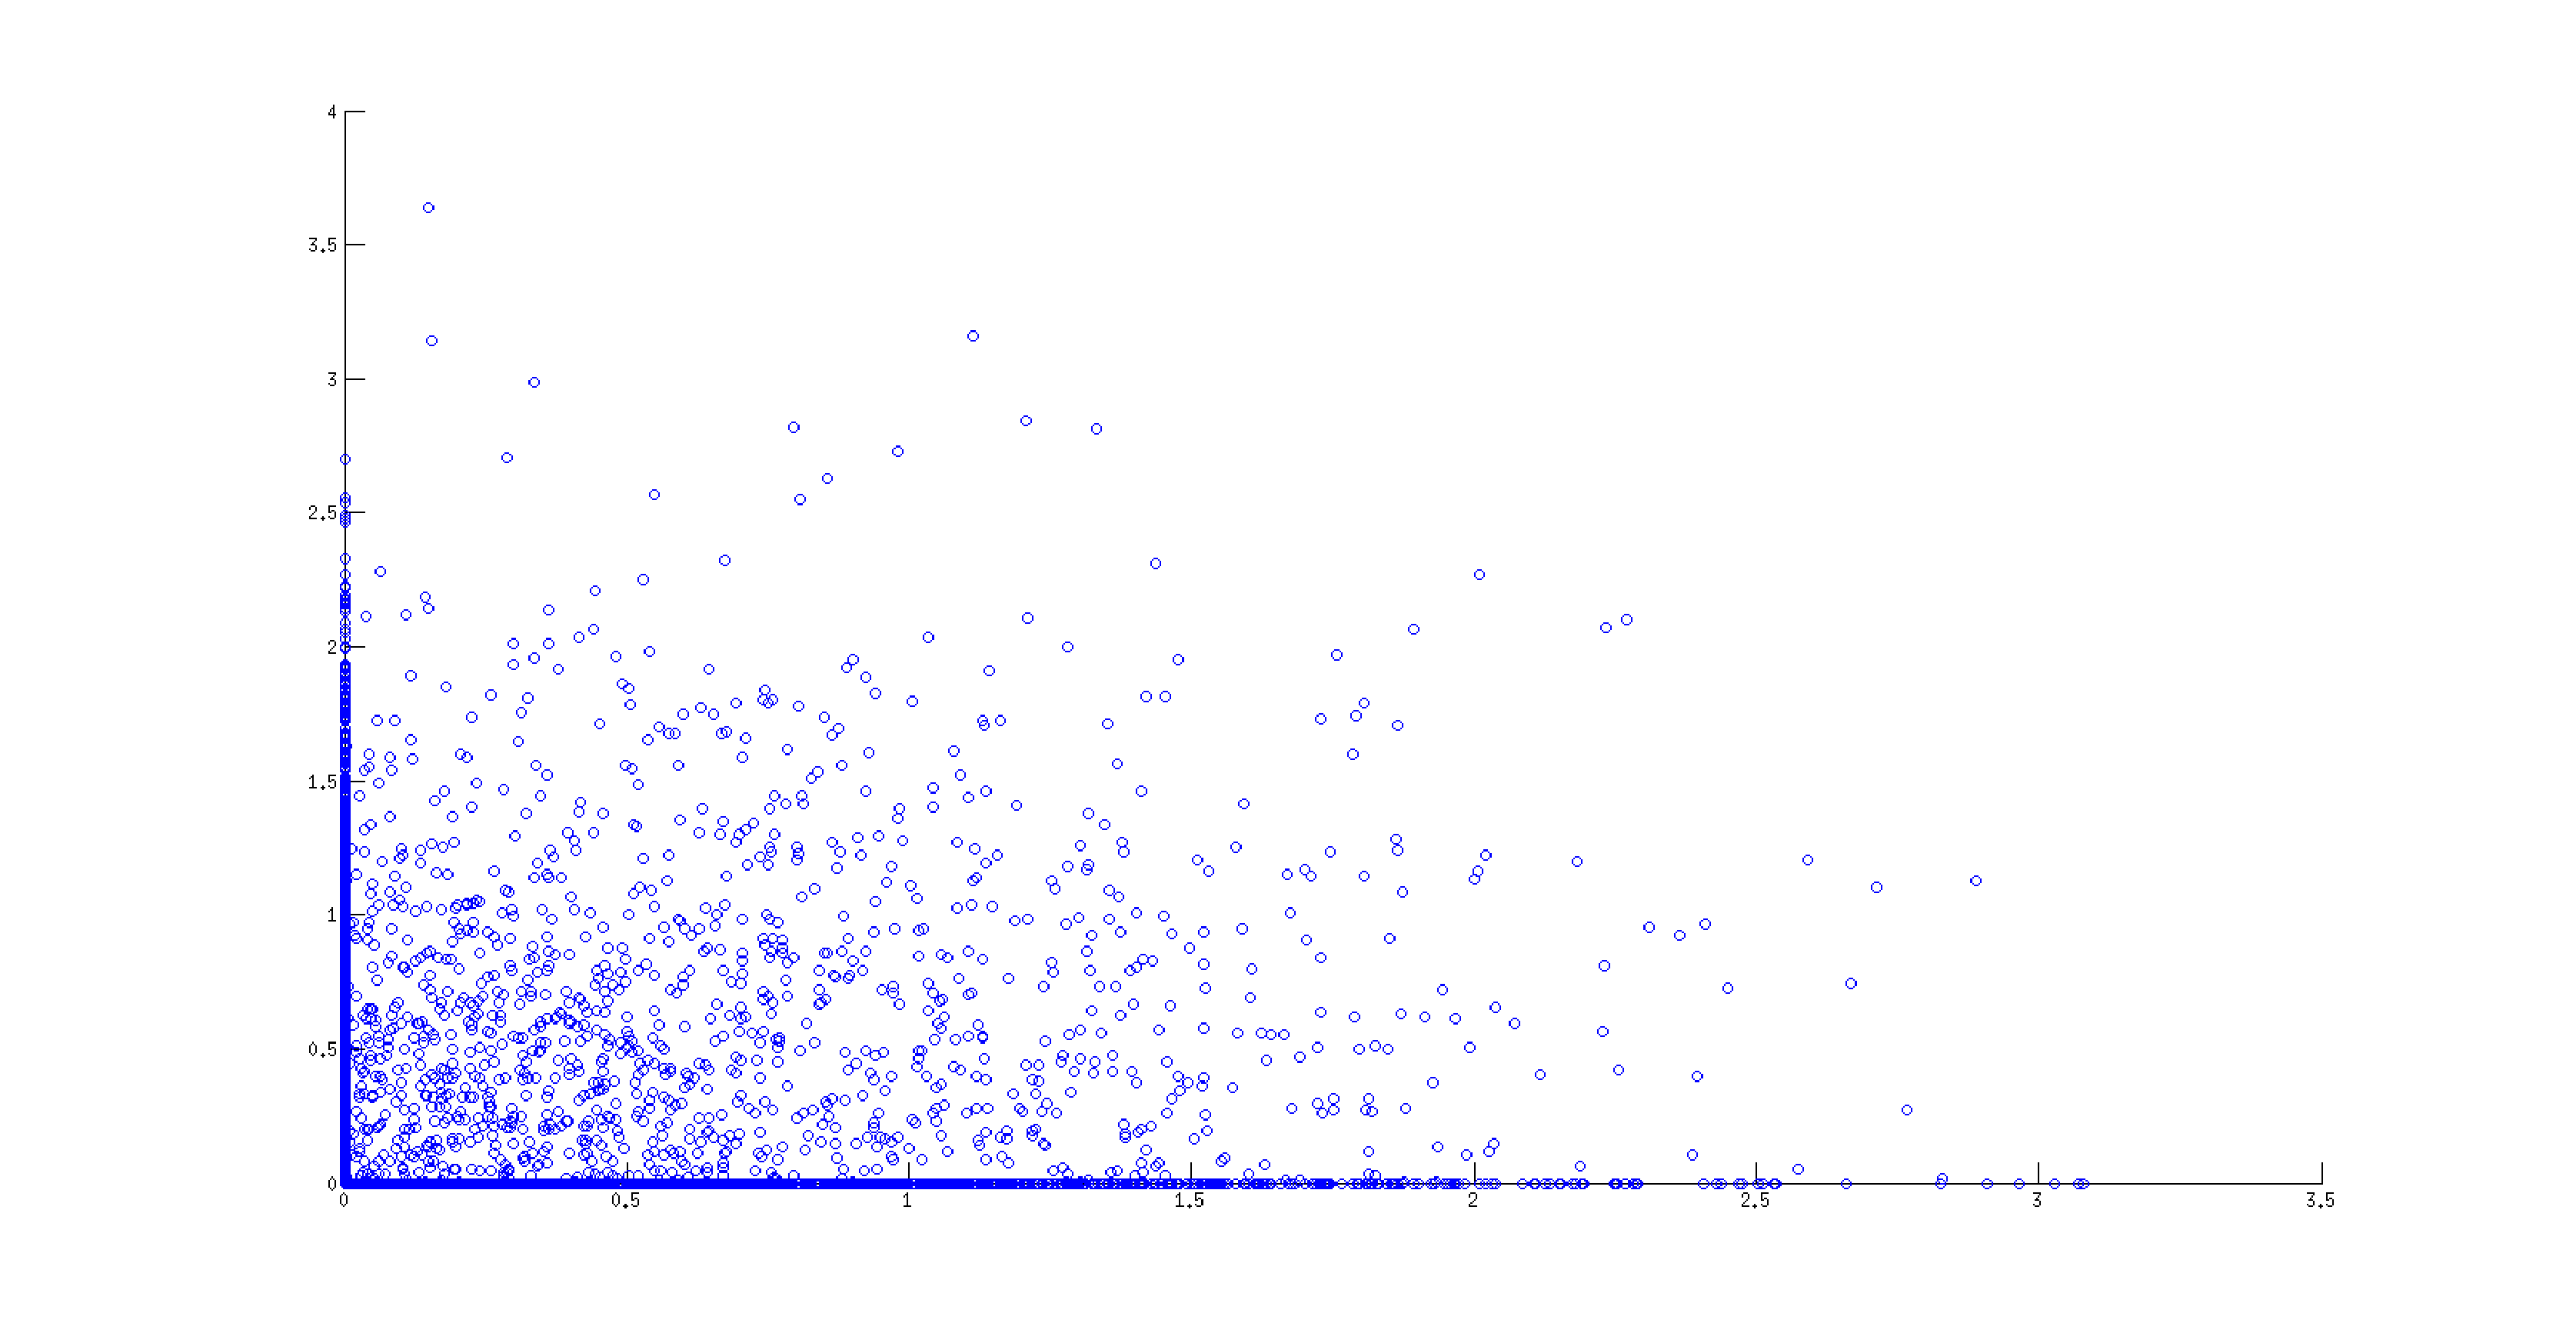
\includegraphics[width=0.9\textwidth]{6b}
\end{center}
\caption{Scatter plot of $f_2$ over $f_1$, for $\mu = -0.5,\rho_v = 0.2$.}
\label{fig:6b}
\end{figure}

\item See Figure~\ref{fig:6c}. 
\begin{figure}[h]
\begin{center}
\includegraphics[width=0.46\textwidth]{6c}
\end{center}
\caption{Plot of $\rho_f$ as a function of $\mu$, for $\rho_v = 0.2$.}
\label{fig:6c}
\end{figure}
\newpage

\item See Figure~\ref{fig:6d}.
\begin{figure}[h]
\begin{center}
\includegraphics[width=0.46\textwidth]{6d}
\end{center}
\caption{Plot of $\rho_f$ as a function of $\mu$, for $\rho_v = 0.9$.}
\label{fig:6d}
\end{figure}

\item See Figure~\ref{fig:6e}.
\begin{figure}[h]
\begin{center}
\includegraphics[width=0.46\textwidth]{6e}
\end{center}
\caption{Plot of $\rho_f$ as a function of $\mu$, for $\rho_v = -0.9$.}
\label{fig:6e}
\end{figure}

\item Thresholding too aggressively kills correlation. As shown in
Figure~\ref{fig:6b}, having a threshold high relative to the mean voltages of
the neurons allows only data points where both neurons displayed high voltage
display correlation; if either neuron fires below the threshold rate, then the
data point is pushed onto the corresponding axis. In particular, this means
that, when both neurons are at low voltage (as strongly correlated neurons
would often be), the data is essentially ignored.
\end{enumerate}
\end{question}

\newpage
\begin{question}{Problem 7}
I took a probabillity class last semester in which I had already done problems
1, 2, 3, and 5, so these were pretty quick. Problem 4 took me a little while to
understand, but was easy once I got the setup straight, and didn't take more
than 15 minutes in all. Problem 6 (the MATLAB simulation) taught me the most.
\end{question}
\end{document}
